\section{Recursive Inverse Dynamics}
\label{sec:invdyn}
As Featherstone pointed out, inverse dynamics can be computed
efficiently by exploiting the recursive structure of an articulated
rigid body system. Such an algorithm greatly reduces the computation
time to linear in the number of links in the articulated system. In
this chapter, we will use our formulation to construct a recursive
inverse dynamics algorithm.

\subsection{Dynamics in the local frame}
For each body link $k$, we define $\vc{c}_k$ as the center of mass in
the local frame and $\vc{d}_{c(k)[i]}$ as the vector between the joint
connecting to the parent link and the joint connecting to the $i$-th child of
link $k$, where $c(k)$ returns the indices of child links of the link
$k$. As a shorthand, we define $\tilde{i} = c(k)[i]$ and use the
notation $\vc{d}_{\tilde{i}}$ hereafter.  Figure \ref{fig:example2}
illustrates the notations using the same structure from the previous
example.

\begin{wrapfigure}{r}{0.6\textwidth}
 \vspace{20pt}
\begin{center}
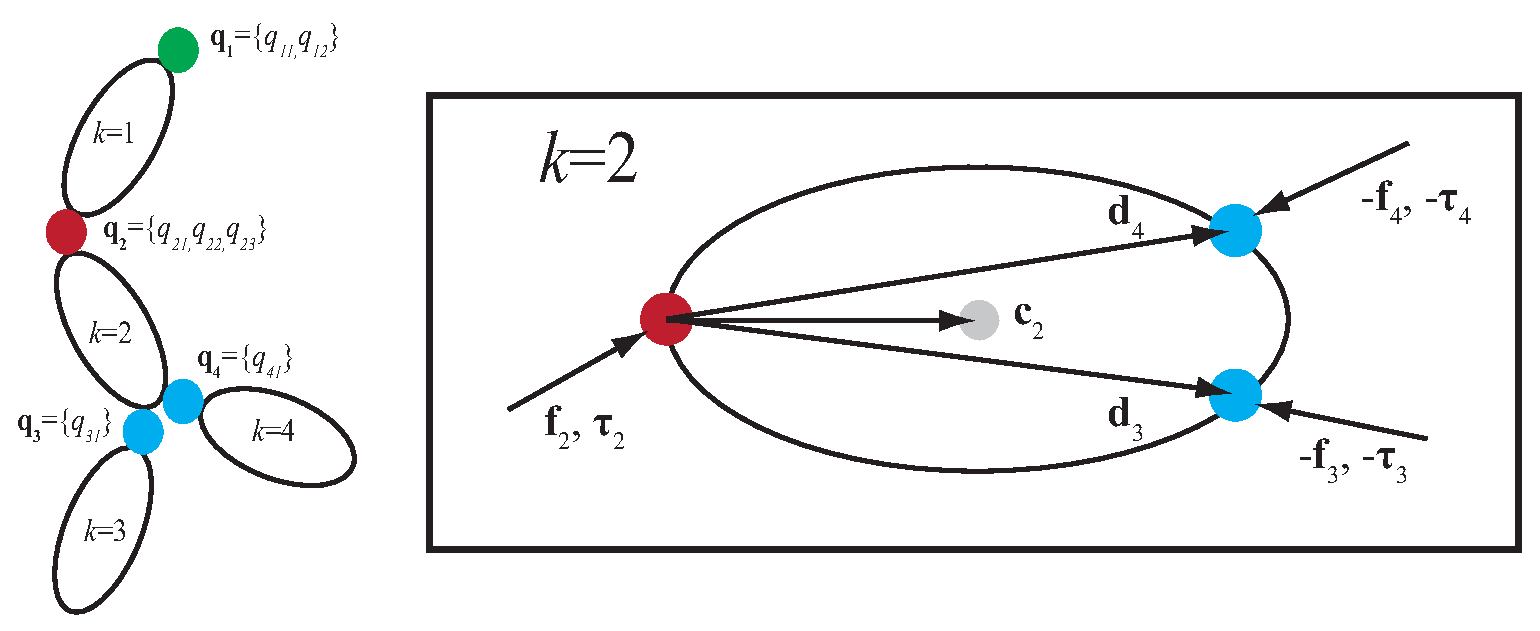
\includegraphics[width=4in]{example2.eps}
\end{center}
\caption{An articulated system.}
 \vspace{0pt}
\label{fig:example2}
\end{wrapfigure}

The goal of the inverse dynamics algorithm is to compute the force and
the torque transmitted between links. For each link $k$, we define the
force and torque received from the parent link $\vc{f}_k$ and
$\bm{\tau}_k$. Similarly, the force and the torque from the $i$-th
child are denoted as $-\vc{f}_{\tilde{i}}$ and
$-\bm{\tau}_{\tilde{i}}$. Please see Figure \ref{fig:example2} for illustration.

To compute these forces and torques, let us first write down
Newton-Euler equations for link $k$ in its local frame. We will use
the notation $\vc{a}_k^\ell$ to denote a vector $\vc{a}$ expressed in
the local frame of link $k$. 
\begin{equation}
\label{eqn:local_newton}
m_k (\dot{\vc{v}}_k)^\ell  =  \vc{f}_k^\ell - \sum_{\tilde{i} \in
  c(k)} \vc{R}_{\tilde{i}}\vc{f}_{\tilde{i}}^\ell 
\end{equation}
\begin{equation}
\label{eqn:local_euler}
\vc{I}_{ck} (\dot{\bm{\omega}}_k)^\ell + \bm{\omega}_k^\ell \times
\vc{I}_{ck} \bm{\omega}_k^\ell =  \bm{\tau}_k^\ell - \vc{c}_k \times
\vc{f}_k^\ell - \sum_{\tilde{i} \in c(k)} (\vc{R}_{\tilde{i}}\bm{\tau}_{\tilde{i}}^\ell +
(\vc{d}_{\tilde{i}} - \vc{c}_k) \times (\vc{R}_{\tilde{i}} \vc{f}_{\tilde{i}}^\ell))
\end{equation}

The inverse dynamics algorithm visits each link twice in two recursive
passes. In the first pass, the velocity and acceleration of each link
is computed and expressed in the local frame. In the second pass,
these terms are plugged into above Newton-Euler equations to compute
forces and torques transmitted between links.

\subsection{Pass 1: Compute velocity and acceleration}
The articulated rigid body system can be represented as a tree
structure, where every link from the root to the leaves will be
visited once in Pass 1. The algorithm is recursive because the
computation at each link depends on the computation of its parent
link. Let us first discuss the computation for a general link and take
care of the special case of the root later in this section.

Assuming the velocity and the acceleration of the parent
link, $\vc{v}_{p(k)}^\ell$, $\bm{\omega}_{p(k)}^\ell$,
$(\dot{\vc{v}}_{p(k)})^\ell$, $(\dot{\bm{\omega}}_{p(k)})^\ell$ , are
already computed from the previous iteration, the COM of the link $k$ in
the world frame is $\vc{W}^0_k \vc{c}_k$. The linear velocity of the
link $k$ in Homogeneous coordinates is then expressed as:
\begin{eqnarray}
\label{eqn:global_vel}
\vc{v}_k &=& \dot{\vc{W}}^0_k \vc{c}_k =  \dot{\vc{W}}^0_{p(k)} \vc{W}_k
\vc{c}_k + \vc{W}^0_{p(k)} \dot{\vc{W}}_k \vc{c}_k \nonumber \\ 
 &=& \dot{\vc{W}}^0_{p(k)} (\vc{c}_{p(k)} + \vc{W}_k \vc{c}_k -
\vc{c}_{p(k)}) + \vc{W}^0_{p(k)} \dot{\vc{W}}_k \vc{c}_k \nonumber \\
&=& \vc{v}_{p(k)} + \dot{\vc{W}}^0_{p(k)} (\vc{W}_k \vc{c}_k -
\vc{c}_{p(k)}) +\vc{W}^0_{p(k)} \dot{\vc{W}}_k \vc{c}_k
\end{eqnarray}
where the fourth element of the vector $\vc{W}_k \vc{c}_k -
\vc{c}_{p(k)}$ and that of the vector $\dot{\vc{W}}_k \vc{c}_k$ are both zero. This will
result in elimination of the translation part of the
transformation. We can therefore express $\vc{v}_k$ in Cartesian space
as:
\begin{eqnarray}
\vc{v}_k &=& \vc{v}_{p(k)} + \dot{\vc{R}}^0_{p(k)} (\vc{R}_k \vc{c}_k
+ \vc{d}_k - \vc{c}_{p(k)}) +\vc{R}^0_{p(k)} \dot{\vc{R}}_k \vc{c}_k \nonumber \\
&=& \vc{v}_{p(k)} + [\bm{\omega}_{p(k)}]\vc{R}^0_{p(k)} (\vc{R}_k
\vc{c}_k + \vc{d}_k -\vc{c}_{p(k)}) +\vc{R}^0_{p(k)}
[\hat{\bm{\omega}}_k]\vc{R}_k \vc{c}_k \mbox{\ \ (Using $[\bm{\omega}] = \dot{\vc{R}} \vc{R}^T$)}
\end{eqnarray}

So far $\vc{v}_k$ is computed in the world frame and we would like to
transform it to the local frame.
\begin{eqnarray}
\vc{v}_k^\ell &=& {\vc{R}_k^0}^T \vc{v}_k = \vc{R}_k^T
{\vc{R}^0_{p(k)}}^T \vc{v}_k \nonumber \\
&=& \vc{R}_k^T (\vc{v}_{p(k)}^\ell + [\bm{\omega}_{p(k)}^\ell] (\vc{R}_k
\vc{c}_k + \vc{d}_k -\vc{c}_{p(k)}) + [\hat{\bm{\omega}}_k] \vc{R}_k
\vc{c}_k) \mbox{\ \ (Using $\vc{R}[\bm{\omega}]\vc{R}^T =
  [\vc{R}\bm{\omega}]$)} \nonumber \\
&=& \vc{R}_k^T (\vc{v}_{p(k)}^\ell + [\bm{\omega}_{p(k)}^\ell]
(\vc{d}_k -\vc{c}_{p(k)})) + \vc{R}_k^T( ([\bm{\omega}_{p(k)}^\ell] + [\hat{\bm{\omega}}_k]) \vc{R}_k
\vc{c}_k) \nonumber \\
&=& \vc{R}_k^T (\vc{v}_{p(k)}^\ell + \bm{\omega}_{p(k)}^\ell \times
(\vc{d}_k -\vc{c}_{p(k)})) + \bm{\omega}_k^\ell \times \vc{c}_k \mbox{\ \ (Using $\vc{R}[\bm{\omega}]\vc{R}^T =
  [\vc{R}\bm{\omega}]$)} 
\end{eqnarray}

Similarly, we can compute the angular velocity of the link $k$ in the
world frame and then transform it to the local frame.
\begin{eqnarray}
[\bm{\omega}_k] &=& \dot{\vc{R}}^0_{k} {\vc{R}^0_k}^T =
(\dot{\vc{R}^0_{p(k)} \vc{R}_k}) (\vc{R}_k^T {\vc{R}^0_{p(k)}}^T) =
\dot{\vc{R}}^0_{p(k)} \vc{R}_k \vc{R}_k^T {\vc{R}^0_{p(k)}}^T +
\vc{R}^0_{p(k)} \dot{\vc{R}}_k \vc{R}_k^T {\vc{R}^0_{p(k)}}^T
\nonumber \\
&=& [\bm{\omega}_{p(k)}] + \vc{R}^0_{p(k)} [\hat{\bm{\omega}}_k ] {\vc{R}^0_{p(k)}}^T
\end{eqnarray}

\begin{eqnarray}
[\bm{\omega}_k^\ell] &=& [{\vc{R}^0_k}^T \bm{\omega}_k] = {\vc{R}^0_k}^T
[\bm{\omega}_k] \vc{R}^0_k \nonumber \\
&=& \vc{R}_k^T ({\vc{R}^0_{p(k)}}^T [\bm{\omega}_{p(k)}] \vc{R}^0_{p(k)}
+ [\hat{\bm{\omega}}_k]) \vc{R}_k = \vc{R}_k^T
([\bm{\omega}_{p(k)}^\ell] + [\hat{\bm{\omega}}_k]) \vc{R}_k \nonumber \\
\bm{\omega}_k^\ell &=& \vc{R}_k^T
(\bm{\omega}_{p(k)}^\ell + \hat{\bm{\omega}}_k)
\end{eqnarray}

Next, we compute the linear and the angular acceleration for the link
$k$. Note that the linear acceleration must be computed in the world
frame first and then transformed into the local frame. If we instead
take the time derivative on $\vc{v}_k^\ell$,
i.e. $\dot{\vc{v}}_k^\ell$, the result is different from the true
linear acceleration $(\dot{\vc{v}}_k)^\ell$, as the former does not
take into account the Colirios force due to the moving frame. 
\begin{eqnarray}
\vc{v}_k &=& \vc{R}^0_k \vc{v}_k^\ell = \vc{R}^0_{p(k)} (\vc{v}_{p(k)}^\ell + \bm{\omega}_{p(k)}^\ell \times
(\vc{d}_k -\vc{c}_{p(k)})) + \vc{R}^0_k \bm{\omega}_k^\ell \times
\vc{c}_k \nonumber \\
(\dot{\vc{v}}_k)^\ell &=& {\vc{R}^0_k}^T \dot{\vc{R}}^0_{p(k)}
(\vc{v}_{p(k)}^\ell + \bm{\omega}_{p(k)}^\ell \times (\vc{d}_k -
\vc{c}_{p(k)})) + \vc{R}_k^T (\dot{\vc{v}}_{p(k)}^\ell +
  \dot{\bm{\omega}}_{p(k)}^\ell \times (\vc{d}_k - \vc{c}_{p(k)}))
  \nonumber \\ &&+
  {\vc{R}^0_k}^T \dot{\vc{R}}^0_k (\bm{\omega}_k^\ell \times \vc{c}_k)
  + \dot{\bm{\omega}}_k^\ell \times \vc{c}_k \nonumber \\
&=& \vc{R}_k^T (\dot{\vc{v}}_{p(k)}^\ell +
\bm{\omega}_{p(k)}^\ell \times \vc{v}_{p(k)}^\ell + \dot{\bm{\omega}}_{p(k)}^\ell \times (\vc{d}_k - \vc{c}_{p(k)}) + \bm{\omega}_{p(k)}^\ell \times (\bm{\omega}_{p(k)}^\ell \times (\vc{d}_k -
\vc{c}_{p(k)}))) \nonumber \\ && + \bm{\omega}_k^\ell \times (\bm{\omega}_k^\ell
\times \vc{c}_k) + \dot{\bm{\omega}}_k^\ell \times \vc{c}_k \mbox{\ \
  (Using ${\vc{R}^0_k}^T \dot{\vc{R}}^0_k = [\bm{\omega}_k^\ell]]$)} \nonumber \\
&=& \vc{R}_k^T ((\dot{\vc{v}}_{p(k)})^\ell + \dot{\bm{\omega}}_{p(k)}^\ell \times (\vc{d}_k - \vc{c}_{p(k)}) + \bm{\omega}_{p(k)}^\ell \times (\bm{\omega}_{p(k)}^\ell \times (\vc{d}_k -
\vc{c}_{p(k)}))) \nonumber \\ && + \bm{\omega}_k^\ell \times (\bm{\omega}_k^\ell
\times \vc{c}_k) + \dot{\bm{\omega}}_k^\ell \times \vc{c}_k \mbox{\ \
  (Using ($\dot{\vc{v}}_{p(k)})^\ell = \dot{\vc{v}}_{p(k)}^\ell +
\bm{\omega}_{p(k)}^\ell \times \vc{v}_{p(k)}^\ell$)} 
\end{eqnarray}

In contrast, the angular acceleration $(\dot{\bm{\omega}}_k)^\ell$ is
the same as $\dot{\bm{\omega}}_k^\ell$.
\begin{equation}
(\dot{\bm{\omega}}_k)^\ell = \vc{R}_k^T
((\dot{\bm{\omega}}_{p(k)})^\ell + \dot{\hat{\bm{\omega}}}_k +
\bm{\omega}_{p(k)}^\ell \times \hat{\bm{\omega}}_k)
\end{equation}

\paragraph{Base case:} The base case of this recursive pass computes
the velocity and the acceleration of the root link. We can simplified
the computation as follows:
\begin{eqnarray}
\vc{v}_0^\ell &=& \bm{\omega}_0^\ell \times \vc{c}_0 \nonumber \\
\bm{\omega}_0^\ell& =& \vc{R}_0^T \hat{\bm{\omega}}_0 \nonumber \\
(\dot{\vc{v}}_0)^\ell &=& \bm{\omega}_0^\ell \times (\bm{\omega}_0^\ell
\times \vc{c}_0) + (\dot{\bm{\omega}}_0)^\ell \times \vc{c}_0 \nonumber \\
(\dot{\bm{\omega}}_0)^\ell &=& \vc{R}_0^T \dot{\hat{\bm{\omega}}}_0
\end{eqnarray}

\paragraph{Translational degrees of freedom:}
So far we assume that the links are connected by only rotational DOFs,
but the formulation can be easily generalized to translational
DOFs. Let us rewrite Equation \ref{eqn:global_vel} with the assumption
that $\vc{W}_k$ has only translational DOFs $\vc{q}_k$, i.e. $\vc{R}_k
= \vc{I}_3$ and $\vc{d}_k = \vc{q}_k$.
\begin{equation}
\vc{v}_k = \vc{v}_{p(k)} + \dot{\vc{R}}^0_{p(k)} (\vc{c}_k
+ \vc{q}_k - \vc{c}_{p(k)}) +\vc{R}^0_{p(k)} \dot{\vc{q}}_k 
\end{equation}

Transforming into the local frame of the link $k$, we get
\begin{equation}
\vc{v}_k^\ell = \vc{v}_{p(k)}^\ell + \bm{\omega}_{p(k)}^\ell \times (\vc{c}_k + \vc{q}_k - \vc{c}_{p(k)}) + \dot{\vc{q}}_k
\end{equation}

The angular velocity and accelerations can be derived in the similar
way.
\begin{eqnarray}
\bm{\omega}_k^\ell &=& \bm{\omega}_{p(k)}^\ell \nonumber \\
\dot{\vc{v}}_k^\ell &=& \dot{\vc{v}}_{p(k)}^\ell +
\dot{\bm{\omega}}_{p(k)}^\ell \times (\vc{c}_k + \vc{q}_k -
\vc{c}_{p(k)}) + \bm{\omega}_{p(k)}^\ell \times \dot{\vc{q}}_k +
\ddot{\vc{q}}_k \nonumber \\
\dot{\bm{\omega}}_k^\ell &=& \dot{\bm{\omega}}_{p(k)}^\ell
\end{eqnarray}

\subsection{Pass 2: Compute force and torque}
The second pass computes forces and torques transmitted
between body links. The algorithm visits each link once from the leaf
nodes to the root. At each iteration, we compute $\vc{f}_k^\ell$
and $\bm{\tau}_k^\ell$, given the velocity and the acceleration computed
by Pass 1 and all the forces and torques from the child
links. Specifically, we will plug $\vc{v}_k^\ell$,
$\bm{\omega}_k^\ell$, $(\dot{\vc{v}}_k)^\ell$,
$(\dot{\bm{\omega}}_k)^\ell$, and all the $\vc{f}_{\tilde{i}}^\ell$ and
$\bm{\tau}_{\tilde{i}}^\ell$ into Equation \ref{eqn:local_newton} and
Equation \ref{eqn:local_euler}.

\paragraph{Base case:} The leaf nodes have no child links connected to
them. Therefore, $\vc{f}_{\tilde{i}}$ and $\bm{\tau}_{\tilde{i}}$ are
zero at each leaf node. Similarly for the root link, $\vc{f}_0$ and
$\bm{\tau}_0$ are zero.

\paragraph{Gravity:}
Instead of treating gravity as an external force, we can consider the
effect of gravity by conveniently offsetting the linear acceleration
of the root link by $-\vc{g}$. 
\begin{equation}
(\dot{\vc{v}}_0)^\ell = \bm{\omega}_0^\ell \times (\bm{\omega}_0^\ell
\times \vc{c}_0) + (\dot{\bm{\omega}}_0)^\ell \times \vc{c}_0 -
\vc{R}_0^T \vc{g}
\end{equation}

This is equivalent to adding a fictitious force, $-m_k \vc{g}$, to
each link.  The rest of the algorithm remains unchanged.
